%%% File encoding: UTF-8
%%% äöüÄÖÜß  <-- keine deutschen Umlaute hier? UTF-faehigen Editor verwenden!

%%% Magic Comments zum Setzen der korrekten Parameter in kompatiblen IDEs
% !TeX encoding = utf8
% !TeX program = pdflatex 
% !TeX spellcheck = de_DE
% !BIB program = biber

\documentclass[bachelor,german,smartquotes]{hgbthesis}
% Zulässige Optionen in [..]: 
%   Typ der Arbeit: diploma, master (default), bachelor, internship 
%   Hauptsprache: german (default), english
%		smartquotes: zur vereinfachten Eingabe von Hochkommas (nur "...")
%%%----------------------------------------------------------

\RequirePackage[utf8]{inputenc}		% bei der Verw. von lualatex oder xelatex entfernen!

\graphicspath{{images/}}    % Verzeichnis mit Bildern und Grafiken
\logofile{logo}				% Logo-Datei = images/logo.pdf (\logofile{}, wenn kein Logo gewünscht)
\bibliography{references}  	% Biblatex-Literaturdatei (references.bib)

%%%----------------------------------------------------------
% Angaben für die Titelei (Titelseite, Erklärung etc.)
%%%----------------------------------------------------------

%%% Einträge für ALLE Arbeiten: -----------------------------
\title{Partielle Lösungen zur allgemeinen Problematik}
\author{Peter A.\ Schlaumeier}
\programname{Universal Computing}
\placeofstudy{Hagenberg}
\dateofsubmission{2019}{07}{28}	% {YYYY}{MM}{DD}

%%% Zusätzlich für eine Bachelorarbeit: ---------------------
\thesisnumber{XXXXXXXXXX-A}   % Stud-ID, z.B. 1310238045-A  
% (A = 1. Bachelorarbeit)
\semester{Sommersemester 2019} 
\coursetitle{Einführung in die Tiefere Problematik 1} 
\advisor{Alois B.~Treuer, Päd.\ Phil.}

%%% Restriktive Lizenformel anstatt CC (nur für Typ master) -
%\strictlicense

%%%----------------------------------------------------------
\begin{document}
%%%----------------------------------------------------------

%%%----------------------------------------------------------
\frontmatter                    % Titelei (röm. Seitenzahlen)
%%%----------------------------------------------------------

\maketitle
\tableofcontents

\chapter{Vorwort} 	% engl. Preface


Dies ist \textbf{Version \hgbDate} der \latex-Dokumentenvorlage für 
verschiedene Abschlussarbeiten an der Fakultät für Informatik, Kommunikation
und Medien der FH Oberösterreich in Hagenberg, die mittlerweile auch 
an anderen Hochschulen im In- und Ausland gerne verwendet wird.

Das Dokument entstand ursprünglich auf Anfragen von Studierenden,
nachdem im Studienjahr 2000/01 erstmals ein offizieller
\latex-Grundkurs im Studiengang Medientechnik und -design an der
FH Hagenberg angeboten wurde. Eigentlich war die Idee, die bereits
bestehende \emph{Word}-Vorlage für Diplomarbeiten "einfach" in
\latex\ zu übersetzen und dazu eventuell einige spezielle
Ergänzungen einzubauen. Das erwies sich rasch als wenig
zielführend, da \latex, \va was den Umgang mit Literatur und
Grafiken anbelangt, doch eine wesentlich andere Arbeitsweise
verlangt. Das Ergebnis ist -- von Grund auf neu geschrieben und
wesentlich umfangreicher als das vorherige Dokument --
letztendlich eine Anleitung für das Schreiben mit \latex, ergänzt
mit einigen speziellen (mittlerweile entfernten) Hinweisen für \emph{Word}-Benutzer.
Technische Details zur aktuellen Version finden sich in Anhang \ref{app:TechnischeInfos}.

Während dieses Dokument anfangs ausschließlich für die Erstellung
von Diplomarbeiten gedacht war, sind nunmehr auch  
\emph{Masterarbeiten}, \emph{Bachelor\-arbeiten} und \emph{Praktikumsberichte} 
abgedeckt, wobei die Unterschiede bewusst gering gehalten wurden.

Bei der Zusammenstellung dieser Vorlage wurde versucht, mit der
Basisfunktionalität von \latex das Auslangen zu finden und -- soweit möglich --
auf zusätzliche Pakete zu verzichten. Das ist nur zum Teil gelungen;
tat\-säch\-lich ist eine Reihe von ergänzenden "Paketen" notwendig, wobei jedoch
nur auf gängige Erweiterungen zurückgegriffen wurde.
Selbstverständlich gibt es darüber hinaus eine Vielzahl weiterer Pakete,
die für weitere Verbesserungen und Finessen nützlich sein können. Damit kann
sich aber jeder selbst beschäftigen, sobald das notwendige Selbstvertrauen und
genügend Zeit zum Experimentieren vorhanden sind.
Eine Vielzahl von Details und Tricks sind zwar in diesem Dokument nicht explizit
angeführt, können aber im zugehörigen Quelltext jederzeit ausgeforscht
werden.

Zahlreiche KollegInnen haben durch sorgfältiges Korrekturlesen und
konstruktive Verbesserungsvorschläge wertvolle Unterstützung
geliefert. Speziell bedanken möchte ich mich bei Heinz Dobler für
die konsequente Verbesserung meines "Computer Slangs", bei
Elisabeth Mitterbauer für das bewährte orthographische Auge und
bei Wolfgang Hochleitner für die Tests unter Mac~OS.

Die Verwendung dieser Vorlage ist jedermann freigestellt und an
keinerlei Erwähnung gebunden. Allerdings -- wer sie als Grundlage
seiner eigenen Arbeit verwenden möchte, sollte nicht einfach
("ung'schaut") darauf los werken, sondern zumindest die
wichtigsten Teile des Dokuments \emph{lesen} und nach Möglichkeit
auch beherzigen. Die Erfahrung zeigt, dass dies die Qualität der
Ergebnisse deutlich zu steigern vermag.

Dieses Dokument und die zugehörigen \latex-Klassen sind seit Nov.\ 2017 auf CTAN%
\footnote{Comprehensive TeX Archive Network} 
als Paket \texttt{hagenberg-thesis} verfügbar unter
%
\begin{itemize}
\item[]\url{https://ctan.org/pkg/hagenberg-thesis}.
\end{itemize}
%
Den jeweils aktuellen Quelltexte sowie zusätzliche Materialien findet man unter
%
\begin{itemize}
\item[]\url{https://github.com/Digital-Media/HagenbergThesis}.%
\footnote{Unter \url{https://github.com/Digital-Media/HagenbergThesis/blob/master/CHANGELOG.md}
sowie genauer unter \url{https://github.com/Digital-Media/HagenbergThesis/commits/master} 
findet man auch eine (früher im Anhang dieses Dokuments enthaltene) chronologische Auflistung der 
Änderungen.}
\end{itemize}



\noindent
Trotz großer Mühe enthält ein Dokument wie dieses immer Fehler und Unzulänglichkeiten
-- Kommentare, Verbesserungsvorschläge und sinnvolle Ergänzungen
sind daher willkommen, am einfachsten als Kommentar oder Fehlermeldung ("Issue") 
auf GitHub oder jederzeit auch per E-Mail an
%
\begin{itemize}
\item[]
Dr.\ Wilhelm Burger, Department für Digitale Medien,\newline
Fachhochschule Oberösterreich, Campus Hagenberg (Österreich)\newline
\nolinkurl{wilhelm.burger@fh-hagenberg.at}
\end{itemize}

\noindent
Übrigens, hier im Vorwort (das bei Diplom- und Masterarbeiten üblich, bei Bachelorarbeiten 
aber entbehrlich ist) kann kurz auf die Entstehung des Dokuments eingegangen werden.
Hier ist auch der Platz für allfällige Danksagungen (\zB an den Betreuer, 
den Begutachter, die Familie, den Hund, \ldots), Widmungen und philosophische 
Anmerkungen. Das sollte man allerdings auch nicht übertreiben und auf 
einen Umfang von maximal zwei Seiten beschränken.




 % Optional. Ggf. weglassen
\chapter{Kurzfassung}

\begin{german}
An dieser Stelle steht eine Zusammenfassung der Arbeit, Umfang
max.\ 1 Seite. 
...
\end{german}		
This document gives a quick, relatively minimal example of the use of
\texttt{uafthesis.cls}, while trying to show its features.

This section is contained in \texttt{abstract.tex}.
			

%%%----------------------------------------------------------
\mainmatter          % Hauptteil (ab hier arab. Seitenzahlen)
%%%----------------------------------------------------------

\chapter{Einleitung}
\label{cha:Einleitung}

\section{Zielsetzung}
Dieses Dokument ist als vorwiegend technische Starthilfe für das
Erstellen einer Masterarbeit (oder Bachelorarbeit) mit \latex
gedacht und ist die Weiterentwicklung einer früheren
Vorlage\footnote{Nicht mehr verfügbar.} für das Arbeiten mit
Microsoft \emph{Word}. Während ursprünglich daran gedacht war, die
bestehende Vorlage einfach in \latex zu übernehmen, wurde rasch
klar, dass allein aufgrund der großen Unterschiede zum Arbeiten
mit \emph{Word} ein gänzlich anderer Ansatz notwendig wurde. Dazu
kamen zahlreiche Erfahrungen mit Diplomarbeiten in den
nachfolgenden Jahren, die zu einigen zusätzlichen Hinweisen Anlass gaben.

Das vorliegende Dokument dient einem zweifachen Zweck: 
\emph{erstens} als Erläuterung und Anleitung, \emph{zweitens} als
direkter Ausgangspunkt für die eigene Arbeit. Angenommen wird,
dass der Leser bereits über elementare Kenntnisse im Umgang mit
\latex verfügt. In diesem Fall sollte -- eine einwandfreie
Installation der Software vorausgesetzt -- der Arbeit nichts mehr
im Wege stehen. Auch sonst ist der Start mit \latex\ nicht
schwierig, da viele hilfreiche Informationen auf den zugehörigen
Webseiten zu finden sind (s.\ Kap.~\ref{cha:ArbeitenMitLatex}).





\section{Warum {\latex}?}

Diplomarbeiten, Dissertationen und Bücher im
technisch-natur\-wissen\-schaft\-lichen Bereich werden
traditionell mithilfe des Textverarbeitungssystems \latex
\cite{Lamport1994, Lamport1995} gesetzt. Das hat gute Gründe, denn
\latex ist bzgl.\ der Qualität des Druckbilds, des Umgangs mit
mathematischen Elementen, Literaturverzeichnissen etc.\
unübertroffen und ist noch dazu frei verfügbar. Wer mit \latex
bereits vertraut ist, sollte es auch für die Abschlussarbeit
unbedingt in Betracht ziehen, aber auch für den Anfänger sollte
sich die zusätzliche Mühe am Ende durchaus lohnen.

Für den professionellen elektronischen Buchsatz wurde früher
häufig \emph{Adobe Framemaker} verwendet, allerdings ist diese
Software teuer und komplex. Eine modernere Alternative dazu ist
\emph{Adobe InDesign}, wobei allerdings die Erstellung
mathematischer Elemente und die Verwaltung von Literaturverweisen
zur Zeit nur rudimentär unterstützt werden.%
\footnote{Angeblich werden aber für den (sehr sauberen) Schriftsatz 
in \emph{InDesign} ähnliche Algorithmen wie in \latex\ verwendet.}

Microsoft \emph{Word} gilt im Unterschied zu \latex, 
\emph{Framemaker} und \emph{InDesign} übrigens nicht als professionelle
Textverarbeitungssoftware, obwohl es immer häufiger auch von
großen Verlagen verwendet wird.%
\footnote{Siehe auch \url{http://latex.tugraz.at/mythen.php}.}
Das Schriftbild in \emph{Word}
lässt -- zumindest für das geschulte Auge -- einiges zu wünschen
übrig und das Erstellen von Büchern und ähnlich großen Dokumenten
wird nur unzureichend unterstützt. Allerdings ist \emph{Word} sehr
verbreitet, flexibel und vielen Benutzern zumindest oberflächlich
vertraut, sodass das Erlernen eines speziellen Werkzeugs wie
\latex\ ausschließlich für das Erstellen einer Abschlussarbeit
manchen verständlicherweise zu mühevoll ist. Es sollte daher
niemandem übel genommen werden, wenn er/sie sich auch bei der Abschlussarbeit
auf \emph{Word} verlässt. Im Endeffekt lässt sich mit etwas
Sorgfalt (und ein paar Tricks) auch damit ein durchaus akzeptables
Ergebnis erzielen. 
Ansonsten sollten auch für \emph{Word}-Benutzer 
einige Teile dieses Dokuments von Interesse sein, insbesondere die
Abschnitte über Abbildungen und Tabellen
(Kap.~\ref{cha:Abbildungen}) und mathematische Elemente
(Kap.~\ref{cha:Mathematik}).


\section{Aufbau der Arbeit}

Hier am Ende des Einleitungskapitels (und nicht
etwa in der Kurzfassung) ist der richtige Platz, um die
inhaltliche Gliederung der nachfolgenden Arbeit zu beschreiben.
Hier sollte man darstellen, welche Teile (Kapitel) der Arbeit
welche Funktion haben und wie sie inhaltlich zusammenhängen. Auch
die Inhalte des \emph{Anhangs} -- sofern vorgesehen -- sollten hier
kurz beschrieben werden.

Zunächst sind in Kapitel \ref{cha:Abschlussarbeit} einige wichtige
Punkte zu Abschlussarbeiten im Allgemeinen zusammengefasst.
Kapitel \ref{cha:ArbeitenMitLatex} beschreibt die Idee und die
grundlegenden technischen Eigenschaften von \latex.
Kapitel \ref{cha:Abbildungen} widmet sich der Erstellung von Abbildungen
und Tabellen sowie der Einbindung von Quellcode.
Mathematische Elemente und Gleichungen sind das Thema in Kapitel \ref{cha:Mathematik} 
\usw
Anhang \ref{app:TechnischeInfos} enthält technische Details zu
dieser Vorlage, 
Anhang \ref{app:cdrom} enthält eine Auflistung von zugehörigen Materialien
auf einem beigelegten Speichermedium, und 
Anhang \ref{app:Fragebogen} zeigt ein Beispiel für die
Einbindung eines mehrseitigen PDF-Dokuments.







\chapter{Die Abschlussarbeit}
\label{cha:Abschlussarbeit}

Jede Abschlussarbeit%
\footnote{Die meisten der folgenden Bemerkungen gelten gleichsam für Bachelor-, Master- und Diplomarbeiten.} 
ist anders und dennoch sind sich gute
Arbeiten in ihrer Struktur meist sehr ähnlich, \va\ bei
technisch-natur\-wissen\-schaft\-lichen Themen. 

\section{Elemente der Abschlussarbeit}

Als Ausgangspunkt bewährt hat sich der folgende Grundaufbau, der natürlich 
vari\-iert und beliebig verfeinert werden kann:
%
\begin{enumerate}
\item \textbf{Einführung und Motivation}: Was ist die Problem- oder Aufgabenstellung und
warum sollte sich jemand dafür interessieren?
\item \textbf{Präzisierung des Themas}: Hier wird der aktuelle Stand der Technik
oder Wissenschaft ("State-Of-The-Art") beschrieben, es werden bestehende
Defizite oder offene Fragen aufgezeigt und daraus die
Stoßrichtung der eigenen Arbeit entwickelt.
\item \textbf{Eigener Ansatz}: Das ist natürlich der Kern der Arbeit. Hier
wird gezeigt, wie die vorher beschriebene Aufgabenstellung gelöst und --
häufig in Form eines Programms%
\footnote{\emph{Prototyp} ist in diesem Zusammenhang ein gerne benutzter Begriff, der im Deutschen
allerdings oft unrichtig dekliniert wird. Richtig ist: der \emph{Prototyp}, des \emph{Prototyps}, dem/den \emph{Protototyp} -- falsch hingegen \zB: des \emph{Prototyp\underline{en}}!
} --
realisiert wird, ergänzt durch illustrative Beispiele.
\item \textbf{Zusammenfassung}: Was wurde erreicht und welche Ziele sind
noch offen geblieben, wo könnte weiter gearbeitet werden?
\end{enumerate}
%
Natürlich ist auch ein gewisser dramaturgischer Aufbau der Arbeit
wichtig, wobei zu bedenken ist, dass der Leser in der Regel nur
wenig Zeit hat und -- anders als etwa bei einem Roman -- seine
Geduld nicht auf die lange Folter gespannt werden darf. Erklären
Sie bereits in der Einführung (und nicht erst im letzten Kapitel),
wie Sie an die Sache herangehen, welche Lösungen Sie vorschlagen
und wie erfolgreich Sie damit waren.

Übrigens, auch Fehler und Sackgassen dürfen (und sollten)
beschrieben werden; ihre Kenntnis hilft oft doppelte Experimente und
weitere Fehler zu vermeiden und ist damit sicher nützlicher als
jede Schönfärberei.
Und natürlich ist es auch nicht verboten, seine eigene Meinung 
in sachlicher Form zu äußern.


\section{Arbeiten in Englisch}
\label{sec:englisch}

Diese Vorlage ist zunächst darauf abgestellt, dass die
Abschlussarbeit in deutscher Sprache erstellt wird. Vor allem bei
Arbeiten, die in Zusammenarbeit mit größeren Firmen oder
internationalen Instituten entstehen, ist es häufig erwünscht,
dass die Abschlussarbeit zu besseren Nutzbarkeit in englischer
Sprache verfasst wird, und viele Hochschulen%
\footnote{Die FH Oberösterreich macht hier keine Ausnahme. 
Der Begriff "Fachhochschule" wird dabei entweder gar nicht
übersetzt oder -- wie im deutschsprachigen Raum mittlerweile üblich -- 
mit \emph{University of Applied Sciences}.
%Die offizielle englische Übersetzung von "Medientechnik und -design"
%ist übrigens \emph{Media Technology and Design}.
} 
lassen dies in
der Regel auch zu.

Beachtet sollte allerdings werden, dass das Schreiben dadurch nicht
einfacher wird, auch wenn einem Worte und Sätze im Englischen
scheinbar leichter "aus der Feder" fließen. Gerade im Bereich
der Informatik erscheint durch die Dominanz englischer
Fachausdrücke das Schreiben im Deutschen mühsam und das Ausweichen
ins Englische daher besonders attraktiv. Das ist jedoch
trügerisch, da die eigene Fertigkeit in der Fremdsprache
(trotz der meist langjährigen Schulbildung) häufig überschätzt wird.
Prägnanz und Klarheit gehen leicht verloren und bisweilen ist das
Resultat ein peinliches Gefasel ohne Zusammenhang und soliden
Inhalt. Sofern die eigenen Englischkenntnisse nicht wirklich gut sind, ist
es ratsam, zumindest die wichtigsten Teile der Arbeit zunächst in
Deutsch zu verfassen und erst nachträglich zu übersetzen. Besondere Vorsicht ist bei der Übersetzung von scheinbar
vertrauten Fachausdrücken angebracht. Zusätzlich ist es immer zu
empfehlen, die fertige Arbeit von einem "native speaker"
korrigieren zu lassen.



Technisch ist, außer der Spracheinstellung und den
unterschiedlichen Anführungszeichen (s.\
Abschn.~\ref{sec:anfuehrungszeichen}), für eine englische Arbeit
nicht viel zu ändern, allerdings sollte Folgendes beachtet werden:
%
\begin{itemize}
\item  Die Titelseite (mit der Bezeichnung "Diplomarbeit" oder "Masterarbeit") 
ist für die einzureichenden Exemplare jedenfalls in \emph{deutsch} zu halten,
auch wenn der Titel englisch ist. 
\item Ebenso muss neben dem
englischen \emph{Abstract} auch eine deutsche \emph{Kurzfassung}
enthalten sein. %
\item Akademische Titel von Personen haben im Englischen offenbar
weniger Bedeutung als im Deutschen und werden daher meist
weggelassen.
\end{itemize}

\chapter{Zum Arbeiten mit \latex}
\label{cha:ArbeitenMitLatex}

\section{Einstieg}
\label{sec:LatexEinstieg}

\latex ist eine in den Naturwissenschaften sehr verbreitete
und mittlerweile klassische Textverarbeitungssoftware für das Erstellen
großer und komplizierter Dokumente mit professionellem Anspruch.
Das Arbeiten mit \latex erscheint -- zumindest für den ungeübten Benutzer -- %
zunächst schwieriger als mit herkömmlichen Werkzeugen für die
Textverarbeitung.

Zum Ersten ist -- im Unterschied zu den meisten gängigen
Text\-ver\-arbei\-tungs\-prog\-ram\-men -- \latex nicht \textsc{Wysiwyg}%
\footnote{"What You See Is What You Get." Es gibt auch 
\textsc{Wysiwyg}-Implementierungen für \latex, 
\zB\ \emph{Scientific WorkPlace} (\url{https://www.mackichan.com/}) oder
\emph{LyX} (\url{https://www.lyx.org/}), 
die aber teuer \bzw\ relativ langsam sind.},
sondern es handelt sich um eine \emph{Markup Lang\-uage} (wie HTML) -- noch dazu
eine für den Anfänger recht komplizierte -- und zugehörige Werkzeuge.
Ungewohnt erscheinen sicher auch die vermeintlich starken
Einschränkungen von \latex,
insbesondere in Bezug auf die Wahl der Schriften und das
Layout. Während anfangs of der Eindruck entsteht, dass diese Rigidität
die eigene Kreativität beschränkt, fällt mit der Zeit auf, dass es gerade
dadurch gelingt, sich stärker auf die Inhalte der Arbeit zu
konzentrieren als auf deren äußere Form. Dass am Ende die Form dennoch stimmt,
ist allerdings nur dann gewährleistet, wenn man sich bei den eigenen Modifikationen
der Formate und Parameter äußerste Zurückhaltung auferlegt, es sei denn,
man ist in der Zwischenzeit bereits selbst zum \latex-\emph{Guru} avanciert.

Insgesamt lohnt sich der Aufwand, wie viele meinen, zumal die Abschlussarbeit
in jedem Fall (mit oder ohne \latex) ein substantielles Stück Arbeit ist.
Allerdings sollte mithilfe von \latex ein professionell aussehendes
Ergebnis einfacher zu erreichen sein und es dürfte wohl auch einiger
Ärger mit Fehlern und Einschränkungen gängiger Software erspart bleiben.
Zudem könnte es durchaus sein, dass sich nebenbei auch das eigene Auge für
die Feinheiten des Buchsatzes (weiter-){\obnh}entwickelt.%
\footnote{Dieses abschließende Textelement wurde übrigens zur Ermöglichung eines 
Zeilenumbruchs nach der Klammer so gesetzt: \texttt{\ldots (weiter-)\{{\bs}optbreaknh\}entwickelt.}
Das Makro \texttt{{\bs}optbreaknh} ("optional break with no hyphen") ist in 
\texttt{hgb.sty} definiert.}


\subsection{Software}
\label{sec:Software}

Zum Arbeiten mit \latex wird -- neben einem Computer -- natürlich Software benötigt. Mussten früher oft die einzelnen Komponenten von \latex mühevoll zusammengesucht und für die eigene Umgebung konfiguriert werden, gibt es mittlerweile für die wichtigsten Plattformen (Windows, Mac~Os, Linux) fertige \latex-Installationen, die ohne weiteres Zutun laufen. Die aktuelle Version von \latex\ ist \LaTeXe\ (sprich "LaTeX zwei e"). 
Zum Arbeiten mit \latex\ werden zwei Dinge benötigt:
%
\begin{itemize}
\item \latex-Installation (Distribution),
\item Texteditor oder Autorenumgebung (Frontend).
%\item PostScript/PDF-Software 
\end{itemize}
%
Sämtliche Komponenten sind kostenlos und für alle gängigen Plattformen verfügbar.


\subsubsection{Windows}
\label{sec:Windows}

Unter \emph{Windows} (XP und höher) hat sich folgendes Setup bewährt,
mit dem \ua auch dieses Dokument erstellt wurde:
%
\begin{itemize}
\item \textbf{\latex-Distribution}: \emph{MikTeX 2.9}\footnote{\url{https://miktex.org/}} oder höher.
MikTeX enthält bereits alle notwendigen Hilfsprogramme, wie beispielsweise \texttt{pdflatex}.

\item \textbf{PDF-Viewer}: \emph{SumatraPDF}.%
\footnote{\url{https://www.sumatrapdfreader.org/}}

\item \textbf{Frontend}: \emph{TeXnicCenter}.%
\footnote{\url{http://www.texniccenter.org/}}
Grundsätzlich kann jeder Texteditor%
\footnote{Unter Windows \zB\ \emph{Notepad++} (\url{https://notepad-plus-plus.org/}).}
verwendet werden, praktischer ist jedoch eine integrierte \latex-Um\-geb\-ung wie TeXnicCenter, die einen auch bei 
der Dateiverwaltung, der Verarbeitung der Dokumente und der Fehlerbehandlung unterstützt.
Eine interessante Alternative bietet die Verwendung von \emph{Eclipse}\footnote{\url{https://www.eclipse.org/}}
als plattformunabhängiges Frontend 
(mit dem \emph{TeXlipse}\footnote{\url{https://projects.eclipse.org/projects/science.texlipse}} Plugin).
\end{itemize}
%
Beim erstem Mal sollten \emph{MikTeX}, \emph{SumatraPDF} und \emph{TeXnicCenter} in genau dieser Reihenfolge installiert werden.

Als Gesamtpaket bietet sich \emph{TeXstudio}\footnote{\url{https://www.texstudio.org/}} an. 
In diesem Fall kann die Installation eines separaten PDF-Viewers entfallen, denn dieser ist in der 
Software bereits enthalten.

\subsubsection{Mac~OS}
\label{sec:MacOs}

Unter Mac~OS~X ist die Referenzdistribution \emph{MacTeX}.%
\footnote{\url{https://www.tug.org/mactex/}} 
Sie enthält neben der TeX-Distribution \emph{TeX Live} auch gängige Editoren wie \emph{TeXWorks} oder \emph{TeXshop}. Mit dem \emph{TeX Live Utility} können Pakete verwaltet und die Distribution auf den neuesten Stand gebracht werden. Als Alternative zu den beiden genannten Editoren steht \emph{TeXnicle}%
\footnote{\url{http://www.bobsoft-mac.de/texnicle/texnicle.html}} zur Verfügung. Er bietet -- ähnlich wie \emph{TeXnicCenter} unter Windows -- einen projektbasierten Workflow an.
Ebenso ist auch \emph{TeXstudio} für Mac~OS~X 10.8 und neuer verfügbar.
Ein PDF-Viewer muss unter Mac~OS~X übrigens nicht extra installiert werden. Alle genannten Editoren beinhalten eine eigene PDF-Vorschau.


\subsubsection{Linux}

Auch unter Linux ist \emph{TeX Live} (\so) eine häufig verwendete TeX-Distri\-bution. 
Als Frontend sind beispielsweise
\emph{Lyx}\footnote{\url{https://www.lyx.org/}},
\emph{Kile}\footnote{\url{https://kile.sourceforge.io/}} und
\emph{Texmaker}\footnote{\url{http://www.xm1math.net/texmaker/}} 
verbreitet.
\emph{TeXstudio} ist ebenfalls für alle gängigen Distributionen über die jeweiligen Paket-Manager erhältlich. Alternativ können die entsprechenden Packages von der Webseite bezogen werden.
In manchen gängigen Linux-Versionen ist bereits eine komplette \latex-Distribution enthalten, sodass im besten Fall überhaupt keine zusätzliche Installation notwendig ist.  


\subsection{Literatur}
\label{sec:literatur}

Es ist müßig, ohne geeignete Literatur mit \latex zu beginnen, selbst
fortgeschrittene Benutzer werden immer wieder auf Hilfe angewiesen
sein. Erfreulicherweise ist sehr viel Nützliches auch online verfügbar.
Gute Startpunkte sind \zB
%
\begin{itemize}
\item \emph{\textrm{\LaTeXe}-Kurzbeschreibung} von Daniel et al.\ \cite{Daniel2018}
\item \emph{The Not So Short Introduction to \textrm{\LaTeXe}}
            von Oetiker et al.\ \cite{Oetiker2018}
\end{itemize}
%
\noindent
Als mittlerweile bereits klassisches Handbuch zu \latex ist
%
\begin{itemize}
  \item \emph{A Guide to \textrm{\LaTeX}} von H.~Kopka und P.~Daly \cite{Kopka2003}
\end{itemize}
%
zu empfehlen, zu dem es für Interessierte auch zwei vertiefende
Zusatzbände in Deutsch gibt. Zahlreiche weitere Dokumente zu
\latex und verwandten Themen finden sich \ua im Rahmen des {\em
Comprehensive TeX Archive Network} (CTAN) auf
\begin{quote}
	\url{https://www.ctan.org/}%
	\footnote{\url{https://www.ctan.org/topic/}}
\end{quote}
%
Besonders nützlich sind auch die
\emph{Comprehensive List of \textrm{\latex} Symbols} \cite{Pakin2017}
und die Beschreibungen wichtiger \latex-Pakete, wie
%
\begin{quote}
  \texttt{babel} \cite{Bezos2018},\newline
  \texttt{graphics}, \texttt{graphicx} \cite{Carlisle2017},\newline
  \texttt{fancyhdr} \cite{Oostrum2019},\newline
  \texttt{caption} \cite{Sommerfeldt2011}.
\end{quote}


\section{Schrift}

In einem \latex-Dokument muss zunächst die verwendete Schriftart festgelegt werden. Im Text können dann mittels diverser Auszeichnungen Textstellen durch eine Änderung des Schriftstils hervorgehoben werden.

\subsection{Schriftarten}

\latex verwendet normalerweise die Schriften der \emph{Computer
Modern}
(CM) Serie, die so wie die \emph{TeX}-Software selbst von Donald Knuth%
\footnote{\url{http://www-cs-faculty.stanford.edu/~uno/}} entwickelt
wurden. Die drei Basis-Schrifttypen der CM-Serie in \latex sind
%
\begin{quote}
\begin{tabular}{lcl}
\textrm{Roman}      & & \verb!\textrm{Roman}!,\\
\textsf{Sans Serif} & & \verb!\textsf{Sans Serif}!,\\
\texttt{Typewriter} & & \verb!\texttt{Typewriter}!.\\
\end{tabular}
\end{quote}
%
\noindent In den Augen vieler Benutzer ist allein die Qualität und
Zeitlosigkeit dieser Schriften ein Grund, \latex für seriöse
Zwecke zu verwenden. Ein weiterer Vorteil der \emph{TeX}-Schriften
ist, dass die unterschiedlichen Schriftfamilien und Schnitte
bezüglich der Größe sehr gut aufeinander abgestimmt sind.

Darüber hinaus können aber in \latex auch beliebige 
\emph{PostScript}-Schrif\-ten (Type 1) verwendet werden, was allerdings in
der Praxis einiges an "Tuning"-Arbeit verlangt. Häufig verwendet
werden \zB\ \emph{Times} und \emph{Palatino}, derzeit ist aber ein Trend 
zurück zu den klassischen CM-Schriften zu beobachten.



\subsection{Texte hervorheben}

Texte können auf unterschiedliche Weise aus dem Fließtext hervorgehoben werden.
\begin{itemize}
%
\item Die Auszeichnung in \textit{Kursivschrift} oder "italic" (\verb!\textit{..}!) ist \va\ zum Hervorheben von
Betonungen und Zitaten geeignet, aber auch für
Produktbezeichnungen, Fremdwörter und Variablen im Text, \zB
%
\begin{quote}
\verb!\textit{Variable}! $\rightarrow$ \textit{Variable}
\end{quote}
%
\item \textsl{Slanted} %
(\verb!\textsl{..}!) bedeutet eine geneigte Schrift und
unterscheidet sich damit deutlich von \textit{Italic}; 
zum Vergleich:
%
\begin{quote}
\verb!\textrm{Daimler-Chrysler}! $\rightarrow$ \textrm{Daimler-Chrysler} \newline%
\verb!\textsl{Daimler-Chrysler}! $\rightarrow$ \textsl{Daimler-Chrysler} \newline%
\verb!\textit{Daimler-Chrysler}! $\rightarrow$ \textit{Daimler-Chrysler}
\end{quote}
%
\item \textbf{Boldface} (\verb!\textbf{..}!) wird \ia\ verwendet für 
\textbf{Überschriften}, Bezeichnungen von \textbf{Abbildungen} und 
\textbf{Tabellen}, im Fließtext aber selten:
%
\begin{quote}
\verb!\textbf{Überschriften}! $\rightarrow$ \textbf{Überschriften}
\end{quote}
%
\item \emph{Emphasize} (\verb!\emph!) %
ist normalerweise gleichbedeutend mit \verb!\textit!, wobei
\verb!\emph! allerdings auch bei geschachtelten
Hervorhebungen und im Bereich anderer Schriftschnitte das
"Richtige" tut: 
%
\begin{quote}
\setlength{\tabcolsep}{0pt}%
\begin{tabular}{lcl}
\verb!\textrm{Du \emph{auch} hier?}! & $\;\rightarrow\;$ &
    \textrm{Du \emph{auch} hier?}
\\
\verb!\textit{Du \emph{auch} hier?}! & $\;\rightarrow\;$ &
    \textit{Du \emph{auch} hier?} 
\\
\verb!\textsl{Du \emph{auch} hier?}! & $\;\rightarrow\;$ & 
    \textsl{Du \emph{auch} hier?}
\\
\verb!\textbf{Du \emph{auch} hier?}! & $\;\rightarrow\;$ & 
    \textbf{Du \emph{auch} hier?}
\\
\verb!\texttt{Du \emph{auch} hier?}! & $\;\rightarrow\;$ & 
    \texttt{Du \emph{auch} hier?}
\end{tabular}
\end{quote}
%
\item \underline{Unterstreichungen} sind ein Relikt aus der 
Schreibmaschinenära und im modernen Schriftsatz
eigentlich \underline{überflüssig}. Sie sollten daher nur in
Ausnahmefällen verwendet werden, \zB
%
\begin{quote}
\verb!\underline{überflüssig}!%
\footnote{Unterstrichene Texte werden zudem nicht automatisch abgeteilt.}
\end{quote}
%
\end{itemize}



\section{Textstruktur}

Zur Strukturierung des eigenen Text stellt \latex eine Reihe von Auszeichnungen zur Verfügung.

\subsection{Absatztrennung}

Absätze werden in {\latex}-Quelltext ausschließlich durch das
Einfügen einer oder mehrerer \textbf{Leerzeilen} voneinander
getrennt, es sind also \emph{keinerlei sonstige Steueranweisungen}
notwendig!
%
\begin{center}
\setlength{\fboxrule}{0.2mm}
\setlength{\fboxsep}{2mm}
\fbox{%
\begin{minipage}{0.9\textwidth}
Besonders die Verwendung von \texttt{\textbackslash\textbackslash} und 
 \texttt{\textbackslash{newline}}
Anweisungen zur Absatztrennung ist ein häufig zu beobachtender \textbf{Fehler}. 
Vor normalen Absätzen auch \emph{nichts} verloren hat die
Anweisung \texttt{\textbackslash{paragraph}\{\}}
-- sie ist in \latex\ (im Unterschied zu HTML)
eine Markierung für Überschriften mit Titel (\su)!
\end{minipage}}
\end{center}

Üblicherweise wird von {\latex} zwischen aufeinanderfolgenden 
Ab\-sätzen \emph{kein} zusätzlicher vertikaler Abstand eingefügt.%
\footnote{Das ist die Standardeinstellung in {\latex} und
natürlich abhängig von der verwendeten Dokumentenklasse, Style
etc.} 
Allerdings wird die
\emph{erste} Zeile jedes Absatzes (mit Ausnahme des ersten Absatzes
eines Abschnitts) eingerückt, um so die Absatzgrenzen deutlich zu
machen. Dieses Schema hat sich nicht nur im traditionellen
Buchsatz bewährt%
\footnote{Wer es nicht glaubt, sollte sein Bücherregal (oder notfalls das seiner Eltern) nach Gegenbeispielen durchsuchen.}
und sollte auch beibehalten werden, es sei denn
es gibt wirklich \emph{sehr} gute Gründe dagegen.
Für alle übrigen Gliederungen im vertikalen Textfluss sind Überschriften (s.\ unten) vorgesehen.

% Note: as of 2017-06-12 the \SuperPar macro has been deactivated
%\SuperPar 
%Manchmal besteht allerdings der Wunsch, etwa zur Verdeutlichung eines inhaltlichen Sprungs \emph{zwischen} zwei Absätzen einen zusätzlichen Abstand einzufügen, ohne dabei eine neue Überschrift zu setzen. Das kann gegebenenfalls (wie vor dem aktuellen Absatz passiert) durch 
%%
%\begin{quote}
%\texttt{{\bs}SuperPar} \emph{Manchmal besteht allerdings der Wunsch, \ldots}
%\end{quote}
%%
%erreicht werden, sollte jedoch sehr sparsam und wirklich \textbf{nur in begründbaren Einzelfällen} verwendet werden.%
%\footnote{Das Makro \texttt{{\bs}SuperPar} ist in \texttt{hgb.sty} definiert.}




\subsection{Überschriften}
\label{sec:ueberschriften}

\latex\ bietet -- abhängig von der verwendeten Dokumentenklasse --
einen Satz vordefinierter Überschriftformate in folgender Ordnung:
%
\begin{quote}
\verb!\part{!\texttt{\em Titel}\verb!}!%
\footnote{\texttt{part} ist für die Gliederung eines
größeren Werks in mehrere Teile vorgesehen und wird üblicherweise
bei einer Abschlussarbeit (und auch in diesem Dokument) nicht
verwendet.}
\newline%
\verb!\chapter{!\texttt{\em Titel}\verb!}! \newline%
\verb!\section{!\texttt{\em Titel}\verb!}! \newline%
\verb!\subsection{!\texttt{\em Titel}\verb!}! \newline%
\verb!\subsubsection{!\texttt{\em Titel}\verb!}! \newline%
\verb!\paragraph{!\texttt{\em Titel}\verb!}! \newline%
\verb!\subparagraph{!\texttt{\em Titel}\verb!}!
\end{quote}
%

\paragraph{Häufiger Fehler:} Bei \verb!\paragraph{}! und
\verb!\subparagraph{}! läuft -- wie in diesem Absatz zu sehen --
der dem Titel folgende Text ohne Umbruch in der selben Zeile
weiter, weshalb im Titel auf eine passende Interpunktion (hier
\zB\ \underline{\texttt{:}}) geachtet werden sollte. Der horizontale Abstand
nach dem Titel allein würde diesen als Überschrift nicht erkennbar
machen.


\subsection{Listen}

Listen sind ein beliebtes Mittel zur Textstrukturierung. In
\latex\ sind -- ähnlich wie in HTML -- drei Arten von formatierten
Listen verfügbar: ungeordnete Auflistung ("Knödelliste"),
geordnete Auflistung (Aufzählung) und Beschreibungsliste
(Description):
%
\begin{verbatim}
    \begin{itemize}     ... \end{itemize}
    \begin{enumerate}   ... \end{enumerate}
    \begin{description} ... \end{description}
\end{verbatim}
%
Listeneinträge werden mit \verb!\item! markiert, bei \texttt{description}-Listen mit \verb!\item[!\texttt{\em titel}\verb!]!. Listen
können ineinander verschachtelt werden, wobei sich bei \texttt{itemize}- und \texttt{enumerate}-Listen die Aufzählungszeichen mit
der Schachtelungstiefe ändern (Details dazu in der
\latex-Dokumentation).


\subsection{Absatzformatierung und Zeilenabstand}

Abschlussarbeiten werden -- wie Bücher -- in der Regel einspaltig und
im Blocksatz formatiert, was für den Fließtext wegen der großen
Zeilenlänge vorteilhaft ist. Innerhalb von Tabellen kommt es
wegen der geringen Spaltenbreite jedoch häufig zu Problemen mit
Abteilungen und Blocksatz, weshalb dort ohne schlechtes
Gewissen zum Flattersatz ("ragged right") gegriffen werden sollte (wie
\zB\ in Tab.~\ref{tab:synthesis-techniques} auf Seite
\pageref{tab:synthesis-techniques}).


\subsection{Fußnoten}
Fußnoten können in \latex\ an beinahe jeder beliebigen Stelle,
jedenfalls aber in normalen Absätzen, durch die Anweisung
%
\begin{quote}
\verb!\footnote{!\texttt{\em Fußnotentext}\verb!}!
\end{quote}
%
gesetzt werden. Zwischen der \verb!\footnote!-Marke und dem davor
liegenden Text sollte grundsätzlich \emph{kein Leerzeichen} entstehen (eventuelle
Zeilen\-um\-brüche mit \verb!%! auskommentieren).
Die Nummerierung und Platzierung der Fußnoten
erfolgt automatisch, sehr große Fußnoten werden notfalls sogar auf
zwei aufeinanderfolgende Seiten umgebrochen.


\subsubsection{Fußnoten in Überschriften}

Auch das ist ab und zu nötig, ist aber \va\ deshalb kein so
einfacher Fall, weil die Fußnote in einer Überschrift nur an Ort
und Stelle aufscheinen darf, nicht aber im \emph{Inhaltsverzeichnis}! Ein
konkretes Beispiel dafür ist die Überschrift zu
Kapitel~\ref{cha:Schluss}, die folgendermaßen definiert ist:
%
\begin{quote}
\begin{verbatim}
\chapter[Schlussbemerkungen]%
        {Schlussbemerkungen%
        \protect\footnote{Diese Anmerkung ....}}%
\end{verbatim}
\end{quote}
%
Dabei ist der erste (optionale) Titel \verb![Schlussbemerkungen]!
der Eintrag im Inhaltsverzeichnis und im Seitenkopf. 
Der zweite (gleich lautende) Titel
\texttt{\{Schlussbemerkungen\}} erscheint auf der aktuellen Seite und
enthält auch den \verb!\footnote{}! Eintrag, der allerdings an
dieser Stelle durch die Direktive \verb!\protect! "geschützt"
werden muss. Die \verb!%!-Zeichen sind hier übrigens notwendig,
um eventuelle Leerzeichen, die durch Zeilenumbrüche im Quelltext
entstehen, zu eliminieren (dieser Trick wird 
in \latex\ häufig benötigt, s.\ Abschn.~\ref{sec:kommentare}). 
Ziemlich kompliziert also, und damit 
ein weiterer Grund, Fußnoten an solchen Stellen überhaupt zu vermeiden.

Generell sollte mit Fußnoten sparsam umgegangen werden, da sie den
Textfluss unterbrechen und den Leser ablenken. Insbesondere
sollten Fußnoten nicht (wie \va\ in manchen
sozialwissenschaftlichen Werken gepflegt) derart lang werden, dass
sie einen Großteil der Seite einnehmen und damit praktisch ein
zweites Dokument bilden.%
\footnote{Das führt bei Dokumenten mit vielen Fußnoten bei manchen Lesern angeblich so weit, dass sie aus Neugier (oder Versehen) regelmäßig bei den Fußnoten zu lesen beginnen und dann mühevoll die zugehörigen, kleingedruckten Verweise im Haupttext suchen.}


\subsection{Querverweise}
\label{sec:querverweise}

Zur Verwaltung von Querverweisen innerhalb eines Dokuments stellt
\latex\ einen sehr einfachen Mechanismus zur Verfügung. Zunächst
muss jede Stelle (Kapitel, Abschnitt, Abbildung, Tabelle etc.)
durch
%
\begin{quote}
\verb!\label{!\texttt{\em key}\verb!}!
\end{quote}
%
markiert werden, wobei \texttt{\em key} ein gültiges \latex-Symbol sein
muss. Damit Labels (die nur Zahlen sind) nicht verwechselt werden,
ist es üblich, sie je nach Bedeutung mit einer unterschiedlichen
Prefix zu versehen, \zB\
%
\begin{quote}
\tabcolsep0pt
\begin{tabular}{ll}
\verb!cha:!\texttt{\em kapitel}   & \ \ldots\ für Kapitel  \\
\verb!sec:!\texttt{\em abschnitt} & \ \ldots\ für Abschnitte (Sections) und Unterabschnitte \\
\verb!fig:!\texttt{\em abbildung} & \ \ldots\ für Abbildungen \\
\verb!tab:!\texttt{\em tabelle}   & \ \ldots\ für Tabellen \\
\verb!equ:!\texttt{\em gleichung} & \ \ldots\ für Formeln und Gleichungen\\
\end{tabular}
\end{quote}
%
\noindent Beispiele:\ \verb!\label{cha:Einleitung}! oder
\verb!\label{fig:Screen-1}!. Mit den Anweisungen
%
\begin{quote}
\verb!\ref{!\texttt{\em key}\verb!}! 
\hspace{1em} oder \hspace{1em} 
\verb!\pageref{!\texttt{\em key}\verb!}!
\end{quote}
%
kann an beliebiger Stelle im Dokument die zu \texttt{\em key} gehörige
Nummer bzw.\ Seitennummer eingesetzt werden, \zB\
%
\begin{quote}
\verb!.. wie in Kap.~\ref{cha:Einleitung} erwähnt ..!\\
\verb!.. der Screenshot auf Seite \pageref{fig:Screen-1} ..!
\end{quote}
%
Übrigens werden die Bezeichnungen \emph{Kapitel} und {\em
Abschnitt} auffallend oft falsch verwendet -- Kapitel haben
ausschließlich "ungebrochene" Nummern:
%
\begin{quote}
\begin{tabular}{ll}
   \textrm{Richtig:\ } & Kapitel 7 oder Abschnitt 2.3.4\\
   \textbf{Falsch:\ }  & Kapitel 7.2 oder Abschnitt 5
\end{tabular}
\end{quote}


\section{Wortabstand und Interpunktion}

Während \latex in vielen Bereichen des Schriftsatzes automatisch das bestmögliche Ergebnis zu erzielen versucht, ist im Bereich der Interpunktion Sorgfalt von Seiten des Autors gefragt.

\subsection{\emph{French Spacing}}

Im englischsprachigen Schriftsatz ist es üblich, nach jedem
Satzende einen gegenüber dem normalen Wortzwischenraum
vergrößerten Abstand einzusetzen. Obwohl dies im Deutschen und
Französischen traditionell nicht so ist, wird es wegen der
verbesserten Lesbarkeit auch hier manchmal verwendet (nicht in diesem
Dokument). Falls die englische ("nicht-französische") Satztrennung mit
zusätzlichem Abstand bevorzugt wird, ist lediglich die Zeile
%
\begin{quote}
\verb!\nonfrenchspacing!
\end{quote}
%
am Beginn des Dokuments einzusetzen. 
In diesem Fall sollte 
aber die Interpunktion innerhalb von
Sätzen (nach .\ und :) sorgfältig beachtet weren. Beispielsweise
schreibt sich "Dr.\ Mabuse" in der Form
%
\begin{quote}
\verb!Dr.\ Mabuse! oder \verb!Dr.~Mabuse!
\end{quote}
%
Im zweiten Beispiel wird mit dem \verb!~! Zeichen zudem ein Zeilenumbruch am Leerzeichen verhindert.


\subsection{Gedanken- und Bindestriche}
\label{sec:gedankenstrich}

Die Verwendung der falschen Strichlängen (mit und ohne
Zwischenraum) ist ganz allgemein eine häufige Fehlerquelle.
Bewusst unterschieden werden sollte zwischen
%
\begin{itemize}
\item kurzen Bindestrichen (wie in "Wagner-Jauregg"), %
\item Minus-Zeichen, \zB\ $-7$ (erzeugt mit \verb!$-7$!), und %
\item echten Gedankenstrichen -- wie hier (erzeugt mit \verb!--!).
\end{itemize}
%
\noindent Für das Setzen von Gedankenstrichen\footnote{Für alle
drei gibt es übrigens auch in \emph{Word} entsprechende
Sonderzeichen.} gibt es eindeutige Konventionen:
%
\begin{enumerate}
\item Im \emph{Deutschen} wird üblicherweise einer von zwei
Leerzeichen umgebener Gedankenstrich%
\footnote{Halbgeviertstrich (\emph{En Dash}).} -- wie hier (in
\latex\ mit {\verb*! -- !}) gesetzt. Dieser wird auch für die Angabe von
Zahlenintervallen (Seiten 12--19) benutzt. 
%
\item In \emph{englischen} Texten wird ein noch längerer
Gedankenstrich\footnote{Geviertstrich (\emph{Em Dash}).} \emph{ohne}
zusätzliche Leerzeichen---\emph{as we should be knowing by now}
(in \latex\ mit {\verb*!---!}) verwendet.
%
\end{enumerate}




\subsection{Kommentare}
\label{sec:kommentare}


Textteile können in \latex\ zeilenweise mit \verb!%! auskommentiert werden. Der einem 
\verb!%!-Zeichen nachfolgenden Text wird bis zum nächsten Zeilenende überlesen:
%
\begin{quote}
\verb!Das wird gedruckt. %Dieser Text wird ignoriert.!
\end{quote}
%
Häufig verwendet werden Kommentarzeichen aber auch zum Ausblenden von 
\emph{white space}, also Leerzeichen und Zeilenumbrüchen.
Folgendes Beispiel zeigt etwa, wie mit \verb!%! am Zeilenende das Entstehen
eines Leerzeichens vor einer nachfolgenden Fußnotenmarke vermieden werden kann:
%
\begin{quote}
\begin{verbatim}
In Österreich isst man sonntags Schnitzel.%
\footnote{Was die allgemein gute Kondition erklärt.}
\end{verbatim}
\end{quote}
%

\begin{sloppypar}
\noindent
Auf ähnliche Weise kann das Entstehen von ungewolltem Absatzzwischenraum durch 
den gezielten Einsatz von Kommentarzeilen vermieden werden, \zB\ vor und nach einem zentrierten
Textabschnitt:
\end{sloppypar}
%
\begin{quote}
\begin{verbatim}
... normaler Text.
%
\begin{center}
   Dieser Test ist zentriert.
\end{center}
%
Und jetzt geht es normal weiter ...
\end{verbatim}
\end{quote}
%
Darüber hinaus bietet die \verb!comment!-Umgebung die Möglichkeit, größere Text\-blöcke
in einem Stück auszublenden:
%
\begin{quote}
\begin{verbatim}
\begin{comment}
Dieser Text ...
   ... wird ignoriert.
\end{comment}
\end{verbatim}
\end{quote}




\subsection{Anführungszeichen (Hochkommas)}
\label{sec:anfuehrungszeichen}

Anführungszeichen sind eine häufige (und oft unbemerkte) Fehlerquelle und auch hier sind die Unterschiede zwischen Deutsch und Englisch (neben anderen Sprachen) zu beachten.


\subsubsection{Variante 1: Hochkommas mit der \latex-Standardeinstellung}

Mit der Standardeinstellung von \latex\ (\dah, \emph{ohne} Verwendung der 
hier hier eingestellten Dokumentenoption \texttt{\texttt{smartquotes}}, \su)
muss die Eingabe von vorderen und hinteren Hochkommas exakt nach den entsprechenden
Konventionen erfolgen.
Hier die korrekte \latex-Notation für englische und deutsche Texte:
%
\begin{quote}
\verb!``English''! $\rightarrow$ ``English'',\\
\verb!"`Deutsch"'! $\rightarrow$ {\glqq}Deutsch{\grqq}.
\end{quote}
%
Man beachte die subtilen typografischen Unterschiede zwischen den beiden Sprachen.%
\footnote{Manche Editoren (\zB\ \textsf{TeXnicCenter}) kann man so einstellen, dass
bei der Eingabe eines einfachen Hochkommas (\texttt{\textquotedbl}) die entsprechenden Zeichenfolge 
\emph{automatisch} (kontext- und sprachabhängig) eingesetzt wird.
Insbesondere in \textsf{Overleaf} ist das derzeit leider nicht möglich.}

\emph{Einfache} Anführungszeichen werden im Englischen analog erzeugt, 
im Deutschen werden dafür hingegen die Makros \verb!\glq! \bzw\ \verb!\grq! 
(German left/right quote) benötigt:
%
\begin{quote}
\verb!`English'! $\rightarrow$ `English',\\
\verb!{\glq}Deutsch{\grq}! $\rightarrow$ {\glq}Deutsch{\grq}.
\end{quote}


\subsubsection{Variante 2: Hochkommas mit der Option \texttt{\bfseries smartquotes}}

Diese Vorlage verwendet mit der Dokumentenoption \texttt{smartquotes}
ein \emph{spezielles Setup}, das auf dem \texttt{csquotes}-Paket%
\footnote{\url{https://ctan.org/pkg/csquotes}}
basiert.
Die korrekte Einsatz von Hochkommas vereinfacht sich damit deutlich, weil
abhängig von der aktuellen Spracheinstellung und der Position des Hochkommas
das jeweils richtige Zeichen eingesetzt wird.
Es genügt hier die Verwendung eines doppelten (geraden) Hochkommas \texttt{\textquotedbl}, wie \zB
%
\begin{quote}
\begin{english}\verb!"English"! $\rightarrow$ "English"\end{english}\ (bei Spracheinstellung \texttt{english}),\\
\verb!"Deutsch"! $\rightarrow$ "Deutsch" (bei Spracheinstellung \texttt{german}).
\end{quote}
%
Dabei ist zu beachten, dass die traditionelle Eingabe von Hochkommas (Variante~1, \so) in diesem Fall \emph{nicht}
zur Verfügung steht. Die gemischte Verwendung von Variante~1 und Variante~2 ist somit
nicht möglich! Es sind mit dieser Einstellung auch alle weiteren "shorthands" des 
\texttt{babel}-Pakets%
\footnote{\url{https://ctan.org/pkg/babel}}
(wie \zB\ \verb!"a!, \verb!"o!, \verb!"u!) \emph{permanent deaktiviert} und diese können
auch lokal nicht reaktiviert werden.%
\footnote{Die hier eingestellte Verwendung des \texttt{\textquotedbl} Zeichens als 
beidseitiges "outer quote" Zeichen gilt -- \va\ in Kombination mit der deutschen Sprache --
als "gefährlich", weil das \texttt{babel}-Paket das gerade Hochkomma für spezielle
\emph{shorthand}-Makros nutzt. Das nehmen wir mutig in Kauf, allerdings sind die 
\texttt{babel}-shorthands im aktuellen Setup generell deaktiviert um Schwierigkeiten 
zu vermeiden.}


\subsubsection{Zusätzliche Features des \texttt{csquotes}-Pakets}
Das (mit der Option \texttt{smartquotes} automatisch geladene)
\texttt{csquotes}-Paket bietet zahlreiche weitere Möglichkeiten zur 
Eingabe von zitierten Texten (Zitaten), insbesondere das Makro
%
\begin{itemize}
\item[] \verb!\enquote{text}!,
\end{itemize}
%
das den angegebenen \texttt{text} in der jeweils korrekten Form (\ua\ abhängig von der Spracheinstellung und
Verschachtelungstiefe) als Zitat auszeichnet, zum Beispiel,
%
\begin{itemize}
\item[] \verb|\enquote{Niemand hat die Absicht, eine Mauer zu bauen!}| 
\item[] $\rightarrow$ \enquote{Niemand hat die Absicht, eine Mauer zu bauen!}
\end{itemize}
%
Der Vorteil dieses Konstrukts wird besonders bei \emph{geschachtelten} Zitaten deutlich, 
wie beispielsweise in
%
\begin{itemize}
\item[] \verb|\enquote{Napoleon sagte nur \enquote{Weiter so!} und ging.}| 
\item[] $\rightarrow$ \enquote{Napoleon sagte nur \enquote{Weiter so!} und ging.}
\end{itemize}
%
Eine weiteres praktisches Feature ist das Makro \verb!\foreignquote!, mit dem man sehr einfach
fremdsprachige Zitate im Text einfügen kann, ohne die Spracheinstellung
explizit verändern zu müssen, \zB%
\footnote{Derzeit sind nur die Spracheinstellungen \texttt{german} und \texttt{english} verfügbar.}
%
\begin{itemize}
\item[] \verb|\foreignquote{english}{And God asked him: |\newline
				\verb|   \enquote{Where is Abel thy brother?} And Cain replied: \ldots}| 
\item[] $\rightarrow$ \foreignquote{english}{And God asked him: \enquote{Where is Abel thy brother?} And Cain replied: \ldots}
\end{itemize}


\section{Abteilen (Silbentrennung, \emph{Hyphenation})}
\label{subsec:layout-abteilen}

Um ein sauberes Schriftbild zu erreichen sind -- speziell im
Deutschen wegen der großen Wortlängen -- Abteilungen unerlässlich.
Die Silbentrennung erfolgt entweder \emph{automatisch} oder \emph{manuell} durch
das Einfügen optionaler Trennzeichen. 


\subsection{Automatischer Zeilenumbruch}

In \latex\ wird grundsätzlich automatisch abgeteilt, wobei die Sprache am
Beginn des Dokuments festgelegt und entsprechende Abteilungsregeln
für den gesamten Text verwendet werden.

Besonders bei schmalen Textspalten kann es vorkommen, dass \latex
keine geeignete Stelle für den Zeilenumbruch findet und den Text
über den rechten Rand hinaus laufen lässt. Das ist durchaus
beabsichtigt und soll anzeigen, dass an dieser Stelle ein Problem
besteht, das durch manuelles Eingreifen repariert werden muss.



\subsection{Manueller Zeilenumbruch}

Generell sollte man gegenüber der automatischen Abteilung
misstrauisch sein und das Endergebnis stets sorgfältig überprüfen.
Vor allem Wörter mit Umlauten oder Bindestrichen (\su) werden in \latex\ 
oft unrichtig abgeteilt.


\paragraph{Optionale Zeilenumbrüche:} 
Bei Bedarf können mit \verb!\-! gezielt zulässige Abteilungspunkte 
definiert werden, wie \zB\ in
%
\begin{itemize}
\item[] \verb!Fach\-hoch\-schul\-kon\-fe\-renz!.
\end{itemize}

\paragraph{Zusammengesetzte Wörter:}
Eine unangenehme Eigenheit von \latex\ ist, dass bei \emph{mit Bindestrichen} verbundenen
Wörtern die einzelnen Wortteile generell \emph{nicht automatisch} getrennt werden!
Das ist \va\ in deutschen Texten recht häufig und somit lästig;
beispielsweise würde \latex\ \emph{keinen} der beiden Teile des Worts 
\begin{itemize}
\item[] \verb!Arbeiter-Unfallversicherungsgesetz!
\end{itemize}
automatisch trennen, sondern ggfs.\ ungebrochen über den Zeilenrand hinausragen
lassen! Auch hier kann natürlich (wie oben gezeigt) durch individuelles 
Einsetzen von \verb!\-! Abhilfe geschaffen werden.
%
%%% weggelassen, weil vermutlich nur verwirrend:
%Eine generelle Lösung bietet das (ohnehin bereits
%geladene) \texttt{babel}-Paket%
%\footnote{\url{http://mirrors.ctan.org/language/german/gerdoc.pdf}} %https://ctan.org/pkg/german
%in der Form
%% 
%\begin{itemize}
%\item[] \verb!Arbeiter"=Unfallversicherungsgesetz!,
%\end{itemize}
%also durch Ersetzung des Bindestrichs mit der Zeichenfolge \verb!"=!.
%Damit wird erreicht, dass \latex\ die Wortteile wie unabhängige Einzelwörter behandelt
%und auch so umbricht.%
%\footnote{Achtung: Diese Möglichkeit ist mit der (hier verwendeten) Dokumentenoption
%\texttt{smartquotes} \emph{nicht} verfügbar, weil damit alle derartigen \texttt{babel} 
%"shorthands" deaktiviert sind (s.\ Abschn.~\ref{sec:anfuehrungszeichen}).}

\paragraph{"Schlampige" Formatierung:}
In echten Problemfällen -- etwa bei Textelementen, die nicht umgebrochen 
werden dürfen oder können -- kann \latex\ dazu veranlasst werden, in einzelnen Absätzen
etwas weniger pingelig zu formatieren. Das wird wie folgt erreicht:
%
\begin{LaTeXCode}[numbers=none]
\begin{sloppypar}
Dieser Absatz wird "schlampig" (sloppy) gesetzt ...
\end{sloppypar}
\end{LaTeXCode}
%
Der allerletzte Rettungsanker ist, die betreffende Passage so umzuschreiben, dass sich ein 
passabler Zeilenumbruch ergibt -- schließlich ist man ja selbst der Autor und 
niemandem (abgesehen vom Betreuer) eine Rechtfertigung schuldig.%
\footnote{Angeblich waren eigenständige Textänderungen durch Schriftsetzer
auch beim früheren Bleisatz durchaus üblich.}



\section{Das \texttt{hagenberg-thesis}-Paket}

Dieses Paket enthält mehrere \latex-Dateien, die 
zum Erstellen dieses Dokuments erforderlich sind:
%
\begin{itemize}
\item \nolinkurl{hgbthesis.cls} (Class-Datei): definiert die 
		Dokumentenstruktur, Layout und den gesamten Vorspann des Dokuments (Titelseite \etc).
\item \nolinkurl{hgb.sty} (Style-Datei): enthält zentrale Definitionen und Einstellungen. 
		Diese Datei wird von \nolinkurl{hgbthesis.cls} automatisch geladen, kann 
		aber grundsätzlich auch für andere Dokumente verwendet werden.
\item Weitere Style-Dateien, die von \nolinkurl{hgbthesis.cls} importiert werden:
    \begin{itemize}
	\item[] \nolinkurl{hgbabbrev.sty} (div.\ Abkürzungen),
    \item[] \nolinkurl{hgbalgo.sty} (Algorithmen),
	\item[] \nolinkurl{hgbbib.sty} (Literaturverwaltung),
	\item[] \nolinkurl{hgbheadings.sty} (Seiten-Header),
	\item[] \nolinkurl{hgblistings.sty} (Code-Listings),
    \item[] \nolinkurl{hgbmath.sty} (Mathematisches).
    \end{itemize}
\end{itemize}


\subsection{Einstellungen}
\label{sec:HagenbergEinstellungen}


Alle (\verb!.tex!) Dokumente dieser Klasse beginnen mit der Anweisung
%
\begin{itemize}
\item[] \verb!\documentclass[!\texttt{\emph{type}},\texttt{\emph{language}}\verb!]{hgbthesis}! 
\end{itemize}
%
Dabei sind die möglichen Optionen für \texttt{\emph{type}} 
%
\begin{itemize}
\item[] \verb!master! (Masterarbeit = \emph{default})
\item[] \verb!diploma! (Diplomarbeit)
\item[] \verb!bachelor! (Bachelorarbeit)
\item[] \verb!internship! (Praktikumsbericht)
\end{itemize}
%
Mit der Option \texttt{\emph{language}} kann die Hauptsprache des Dokuments spezifiziert werden, 
die möglichen Werte dafür sind
%
\begin{itemize}
\item[] \verb!german! (\emph{default})
\item[] \verb!english!
\end{itemize}
%
Wird keine Option angegeben, lautet die Standardeinstellung \texttt{[master,german]}.
Der vollständige Quelltext für eine entsprechende \verb!.tex! Hauptdatei ist in Anhang \ref{app:latex} 
gelistet.


\subsubsection{Angaben zur Arbeit}

Die Dokumentenklasse ist für verschiedene Arten von Arbeiten vorgesehen, die sich nur im Aufbau 
der Titelseiten unterscheiden. 
Abhängig vom gewählten Dokumententyp sind unterschiedliche Elemente für die Titelseiten erforderlich (siehe Tabelle \ref{tab:TitelElemente}).
Folgende Basisangaben sind für \textbf{alle} Arten von Arbeiten
erforderlich:
%
\begin{itemize}
\item[] %
\verb!\title{!\texttt{\em Titel der Arbeit}\verb!}! \newline%
\verb!\author{!\texttt{\em Autor}\verb!}! \newline%
\verb!\programname{!\texttt{\em Studiengang}\verb!}! \newline%
\verb!\placeofstudy{!\texttt{\em Studienort}\verb!}! \newline%
\verb!\dateofsubmission{!\texttt{\em yyyy}\verb!}{!\texttt{\em mm}\verb!}{!\texttt{\em dd}\verb!}!
\end{itemize}
%
\noindent Für \textbf{Bachelorarbeiten} werden zusätzlich zu den Basisangaben folgende Elemente verwendet (bei Diplom- und Masterarbeiten nicht relevant):
%
\begin{itemize}
\item[] \verb!\thesisnumber{!\texttt{\em laufende Nummer der Arbeit}\verb!}!%
\footnote{Wird normalerweise von der Institution vergeben. An der
Fakultät Hagenberg ist dies bei einer Bachelorarbeit die (10-stellige) Studenten-ID 
des Autors oder der Autorin,
\zB\ \textsf{0310238045-A} für die erste Bachelorarbeit.} \newline%
\verb!\coursetitle{!\texttt{\em Gegenstand oder Projektlehrveranstaltung}\verb!}! \newline%
\verb!\semester{!\texttt{\em Semester der Lehrveranstaltung}\verb!}! \newline%
\verb!\advisor{!\texttt{\em Name des Betreuers/der Betreuerin}\verb!}!
\end{itemize}

\noindent Für \textbf{Praktikumsberichte} werden zusätzlich zu den Basisangaben folgende
Elemente berücksichtigt:
%
\begin{itemize}
\item[] %
\verb!\thesisnumber{!\texttt{\em laufende Nummer der Arbeit}\verb!}!%
%\footnote{Wird normalerweise von der Institution vergeben. An der
%FH-Hagenberg ist dies bei einer Bachelorarbeit üblicherweise die Matrikelnummer 
%des Autors,
%gefolgt von der Kennzeichnung \textbf{A} (fachbezogene Arbeit) 
%oder \textbf{B} (Praktikumsbericht),
%\zB\ \textsf{238-003-045}.} 
\newline%
\verb!\advisor{!\texttt{\em Betreuer oder Betreuerin im Unternehmen}\verb!}! \newline%
\verb!\companyName{!\texttt{\em Name und Adresse der Firma}\verb!}! \newline%
\verb!\companyPhone{!\texttt{\em Telefonnummer der Firma}\verb!}! \newline%
\verb!\companyUrl{!\texttt{\em Website der Firma}\verb!}!
\end{itemize}

\begin{table}
\caption{Elemente in Titelseiten für verschiedene Dokumentenoptionen.}
\label{tab:TitelElemente}
\centering\small
\begin{tabular}{lcccc}
\emph{Element} & 
\texttt{diploma} &
\texttt{master} &
\texttt{bachelor} & 
\texttt{internship} 
\\
\hline
\verb!\title! 			& $+$ & $+$ & $+$ & $+$ \\
\verb!\author! 			& $+$ & $+$ & $+$ & $+$ \\
\verb!\programname! & $+$ & $+$ & $+$ & $+$ \\
\verb!\placeofstudy! 	& $+$ & $+$ & $+$ & $+$ \\
\verb!\dateofsubmission! 	& $+$ & $+$ & $+$ & $+$ \\
\verb!\thesisnumber! 			& $-$ & $-$ & $+$ & $+$ \\
\verb!\coursetitle! 	& $-$ & $-$ & $+$ & $-$ \\
\verb!\advisor! 		& $-$ & $-$ & $+$ & $+$ \\
\verb!\companyName! 			& $-$ & $-$ & $-$ & $+$ \\
\verb!\companyPhone! 	& $-$ & $-$ & $-$ & $+$ \\
\verb!\companyUrl! 	& $-$ & $-$ & $-$ & $+$ \\
\hline
\end{tabular}
\end{table}



\subsubsection{Titelseiten}

Die ersten Seiten der Arbeit, einschließlich der Titelseite,
werden durch die Anweisung
\begin{itemize}
\item[] \verb!\maketitle!  
\end{itemize}
automatisch generiert, abhängig vom Typ der Arbeit und den obigen
Einstellungen:
%
\begin{center}
\begin{tabular}{cll}
\emph{Seite} & \emph{Master-/Diplomarbeit} & \emph{Bachelorarbeit} \\
  \hline
  \textrm{i} & Titelseite & Titelseite \\
  \textrm{ii} & Copyright-Seite & Betreuerseite \\
  \textrm{iii} & Eidesstattliche Erklärung & Eidesstattliche Erklärung \\
  \hline
\end{tabular}
\end{center}
%
Auf der Copyright-Seite werden auch die Bedingungen für die Nutzung 
und Weitergabe der Arbeit vermerkt. Der zugehörige Text kann durch
folgenden Einstellungen am Beginn des Dokuments bestimmt werden:
%
\begin{description}
\item[\normalfont\texttt{{\bs}cclicense}] ~ \newline
	Veröffentlichung unter einer Creative Commons%
	\footnote{\url{http://creativecommons.org/licenses/by-nc-nd/3.0/}}
	Lizenz, die die freie Weitergabe der Arbeit unter Nennung des Autors, jedoch
	keine kommerzielle Nutzung oder Bearbeitung erlaubt
	(Standardeinstellung).
\item[\normalfont\texttt{{\bs}strictlicense}] ~ \newline 
	Traditionelle Einschränkung der Nutzungsrechte 
	(\emph{Alle Rechte vorbehalten} \bzw\ \emph{All Rights Reserved}).
\item[\normalfont\texttt{{\bs}license\{\emph{Lizenztext}\}}] ~ \newline
	Damit kann alternativ ein eigener \texttt{\emph{Lizenztext}} angegeben werden, 
	falls notwendig. Solche Änderungen sollten natürlich unbedingt mit seiner 
	Hochschule abgestimmt werden.
\end{description}





\subsection{Definierte Abkürzungen}

Es wird im \texttt{hagenberg-thesis}-Paket weiters eine Reihe von Abkürzungsmakros%
\footnote{In Anlehnung an den \texttt{jkthesis}-Style von J.
Küpper (\url{https://ctan.org/pkg/jkthesis}).} definiert, die das
Schreiben vereinfachen und für konsistente
Zwisch\-en\-ab\-stän\-de sorgen (Tab.~\ref{tab:abkuerzungen}).
Bei der Verwendung von Makros ist allgemein zu beachten, dass sie nachfolgende Leerzeichen manchmal
"auffressen", sodass vor dem nachfolgenden Text kein Abstand erzeugt wird.%
\footnote{Bei fast allen in \texttt{hgb.sty} definierten Makros wird dies allerdings durch den Einsatz von \texttt{\textbackslash xspace} verhindert.} 
Dies kann notfalls mit einem nachfolgenden
"\verb!\ !" oder umhüllenden \verb!{}!-Klammern verhindert werden.
%, wie in folgendem (nicht sehr schönen) Beispiel:
%
%\begin{itemize}
%\item[] \verb!Mopeds und Autos haben \ia zwei {\bzw} vier Räder.!\\
      %Mopeds und Autos haben \ia zwei {\bzw} vier Räder.
%\end{itemize}
Bei Verwendung von Makros mit abschließendem Punkt an einem Satzende 
sollte auch darauf geachtet werden, dass keine \emph{doppelten} Punkte gesetzt werden.


\begin{table}
\caption{In \texttt{hgbabbrev.sty} definierte Abkürzungsmakros.}
\label{tab:abkuerzungen}
\centering
\begin{tabular}{llp{2cm}ll}
\hline
    \verb+\bzw+        & \bzw   & &  \verb+\ua+         & \ua \\
    \verb+\bzgl+       & \bzgl  & &  \verb+\Ua+         & \Ua \\
    \verb+\ca+         & \ca    & &  \verb+\uae+        & \uae \\
    \verb+\dah+        & \dah   & &  \verb+\usw+        & \usw \\
    \verb+\Dah+        & \Dah   & &  \verb+\uva+        & \uva \\
    \verb+\ds+         & \ds    & &  \verb+\uvm+        & \uvm \\
    \verb+\evtl+       & \evtl  & &  \verb+\va+         & \va \\
    \verb+\ia+         & \ia    & &  \verb+\vgl+        & \vgl \\
    \verb+\sa+         & \sa    & &  \verb+\zB+         & \zB \\
    \verb+\so+         & \so    & &  \verb+\ZB+         & \ZB \\
    \verb+\su+         & \su    & &  \verb+\etc+        & \etc \\
\hline
\end{tabular}
\end{table}




\subsection{Sprachumschaltung}
\label{sec:sprachumschaltung}

Für englischsprachige Abschnitte (\zB\ das Abstract oder englische
Zitate) sollte die \emph{Sprache} von Deutsch auf Englisch
umgeschaltet werden, um die richtige Form der Silbentrennung zu
erhalten. Damit nicht versehentlich auf das Rückstellen der
Sprache vergessen wird, sind dafür im \texttt{hagenberg-thesis}-Paket zwei
spezielle \emph{Environments} vorgesehen:
%
\begin{itemize}
\item[] 
\verb!\begin{english}!\\
\verb!    This is a 1-page (maximum) summary!\\
\verb!    of your work in English.!\\
\verb!\end{english}!
\end{itemize}

\begin{itemize}
\item[] 
\verb!\begin{german}!\\
\verb!    Text in Deutsch (wenn die Hauptsprache!\\
\verb!    auf Englisch gesetzt ist).!\\
\verb!\end{german}!
\end{itemize}
%
Zur Kontrolle lässt sich die aktuelle Spracheinstellung mit dem Makro \verb!\languagename!
anzeigen. An dieser Stelle ergibt das etwa "\texttt{\languagename}" (\emph{new german}, \dah\ neue deutsche Rechtschreibung).


\subsection{Zusätzliche {\latex}-Pakete}

Für die Verwendung dieses Dokuments ist eine Reihe von
zusätzlichen \latex-Paketen erforderlich
(Tab.~\ref{tab:packages}). Diese Pakete werden am Anfang
durch das \texttt{hagenberg-thesis}-Paket automatisch geladen. 
Alle verwendeten Pakete sind
Teil der \latex\ Standard-Installation, wie \zB in MikTeX, wo
auch entsprechende Dokumentation gefunden werden kann (meist als DVI-Dateien).
Die aktuellen Versionen der Pakete sind online verfügbar, \ua\ auf den
in Abschn.~\ref{sec:literatur} angegebenen CTAN-Sites.

\begin{table}
\caption{Die wichtigsten der im \texttt{hagenberg-thesis}-Paket verwendeten \latex-Ergänzungen. 
Alle sind in den gängigen \latex\ Standardinstallationen (\zB MikTeX) bereits enthalten.}
\label{tab:packages}
\centering\small\tabcolsep2pt
\begin{tabular}{ll}
%\hline
\emph{Paket} &  \emph{Funktion} \\
\hline
\texttt{algorithmicx} & Beschreibung von Algorithmen \\ 
\texttt{amsfonts}, \texttt{amsbsy}   &  Mathematische Symbole \\ 
\texttt{amsmath}  &  Mathematischer Schriftsatz \\ 
\texttt{babel}  	&  Sprachumschaltung \\ 
%\texttt{babelbib} &  Mehrsprachige Literaturverwaltung \\ 
\texttt{biblatex} &  Literaturverwaltung \\ 
\texttt{caption}  &  Flexiblere Captions \\ 
\texttt{cite}     &  Sortierte Literaturverweise \\ 
\texttt{color}    &  Farbige Textelemente und Hintergrundfarben \\ 
%\texttt{eurosym}  &  {\euro}-Symbol (\verb!\euro!)\\ 
\texttt{marvosym}  &  {\euro}-Symbol (\verb!\euro!)\\ 
\texttt{exscale}  &  Korrekte Schriftgrößen im Math-Modus \\ 
\texttt{fancyhdr} &  zur Gestaltung Kopfzeilen (header) \\ 
\texttt{float}    &  Verbessertes Float-Handling \\ 
\texttt{fontenc}  &  zur Verwendung der cm-super Type1 Postscript Schriften \\ 
\texttt{graphicx} &  Einbindung von EPS-Grafiken \\ 
\texttt{hyperref} &  erzeugt aktive Querverweise im PDF-Dokument \\ 
\texttt{ifthen}   &  für logische Entscheidungen in \latex\\
\texttt{inputenc} &  Erweiterter Eingabezeichensatz \\ 
%\texttt{latin1}   &  T1-Schriften, \ua zur besseren Silbentrennung \\ 
\texttt{listings} &  Auflistung von Programmcode \\ 
%\texttt{ngerman}  &  Neue deutsche Rechtschreibung \\ 
\texttt{upquote}  &  Gerade Hochkommas in \texttt{verbatim}-Texten \\ 
\texttt{url}      &  Behandlung von URLs im Text \\ 
\texttt{verbatim} &  Verbesserte \texttt{verbatim}-Umgebung \\
\texttt{csquotes}    &  Kontextabhängige Hochkommas \\ 
\hline
\end{tabular}
\end{table}





\section{\latex-Fehlermeldungen und Warnungen}

Während des Durchlaufs gibt \latex\ Unmengen von
Meldungen aus, die einen in ihrer Fülle zunächst nicht verwirren
sollten, \zB:

\begin{scriptsize}
\begin{verbatim}
...
Overfull \hbox (14.43593pt too wide) in paragraph at lines 105--109
\OT1/cmr/m/n/10.95 F[]ur die Ein-bin-dung von Gra-phi-ken in L[]T[]X wird die V
er-wen-dung des Standard-
[10] [11]
Overfull \hbox (5.01222pt too wide) in paragraph at lines 148--154
\OT1/cmr/m/n/10.95 wen-di-gen Ras-te-rung kei-nen Sinn, auch bei 1200 dpi-Druck
ern. Spe-zi-ell \OT1/cmr/m/it/10.95 Screen-
...
\end{verbatim}
\end{scriptsize}
%
\emph{Errors} (Fehler) müssen korrigiert werden, wobei einem \latex\ diese Arbeit 
nicht leicht macht, da manchmal (\zB\ wenn eine schließende Klammer \verb!}! 
vergessen wurde) das Problem erst viel später im Text lokalisiert wird.
In solchen Fällen kann es nützlich sein, das erzeugte Ausgabedokument
zu inspizieren um festzustellen, ab welcher Stelle die Ergebnisse
aus dem Ruder laufen.  
Bei kapitalen Fehlern bleibt der \latex-Prozessor überhaupt stehen und 
erzeugt keine Ausgabe (in Verbindung mit einer meist kryptischen
Fehlermeldung) -- hier hilft meist nur eine genaue
Analyse des Quelltexts oder der gerade zuvor durchgeführten Schritte.
Ein ausführliches Fehlerprotokoll findet sich jeweils in der \verb!.log!-Datei 
des Hauptdokuments.

Falls keine Fehler mehr angezeigt werden, ist zumindest die syntaktische Struktur
des Dokuments in Ordnung.
Genauer ansehen sollte man sich die Liste von Meldungen jedoch
spätestens beim Abschluss der Arbeit, um übrig gebliebene Probleme, wie
überlange Textzeilen, unaufgelöste Verweise und ähnliche zu
beseitigen.
Am Ende sollte das Ergebnis jedenfalls so ausehen:
%
\begin{quote}
\verb!LaTeX-Result: 0 Error(s), 0 Warning(s), ...!
\end{quote}
\chapter{Abbildungen, Tabellen, Quellcode}
\label{cha:Abbildungen}



\chapter[Mathem.\ Formeln etc.]{Mathematische Formeln, Gleichungen und Algorithmen}
\label{cha:Mathematik}


%
% bgteubner class bundle
%
% literatur.tex
% Copyright 2003--2012 Harald Harders
%
% This program may be distributed and/or modified under the
% conditions of the LaTeX Project Public License, either version 1.3
% of this license or (at your opinion) any later version.
% The latest version of this license is in
%    http://www.latex-project.org/lppl.txt
% and version 1.3 or later is part of all distributions of LaTeX
% version 1999/12/01 or later.
%
% This program consists of all files listed in manifest.txt.
% ===================================================================
%
\bibliographystyle{bgteupln}
%\bibliographystyle{bgteupln2}
%\bibliographystyle{bgteuabbr}
%\bibliographystyle{bgteuabbr2}
\bibliography{literatur}

% ===================================================================

\chapter{Drucken der Abschlussarbeit}
\label{cha:Drucken}




\section{PDF-Workflow}
\label{sec:pdf}

In der aktuellen Version wird \latex\ so benutzt, dass damit direkt PDF-Dokumente (ohne den früher üblichen Umweg über DVI und PS) erzeugt werden.
Zur Arbeit mit dem Sumatra PDF-Viewer unter Windows und TeXnicCenter ist ein passendes Ausgabeprofil vorbereitet
(s.\ Abschn.\ \ref{sec:VerwendungUnterWindows} im Anhang).%



\begin{comment}

\section{DVI-PS-Workflow (optional)}

Dieser Abschnitt ist nur dann relevant, wenn \latex\ im ("alten") "Kompatibilitätsmodus" verwendet wird,
in dem die druckfähige PDF-Datei über DVI- und PostScript-Zwischendateien erzeugt wird. 
Dieser Modus ist weiterhin notwendig, wenn das \texttt{psfrag}-Package verwendet wird
(s.\ Abschnitt \ref{sec:psfrag}).

\subsection{DVI-Dateien}

\latex selbst erzeugt sogenannte DVI-Dateien (\emph{device independent}), die man mit einem
DVI-\emph{Viewer} wie
\zB\ \texttt{Yap}%
\footnote{\emph{Yet Another Previewer} von Christian Schenk, Teil der
MikTeX-Installation.}
betrachten und auch drucken kann. Falls das Dokument EPS-Grafiken
enthält, muss auch \emph{GhostScript} installiert sein, um Bilder und Grafiken im DVI-Previewer 
direkt betrachten zu können.%
\footnote{In den aktuellen MikTeX-Installationen ist eine spezielle Version von GhostScript (\texttt{mgs.exe}) für die interne Darstellung von Grafiken in YAP bereits enthalten.}



\subsection{PostScript- und PDF-Dateien}

PostScript-Dateien erzeugt man mit dem Programm \texttt{dvips}, das Teil der
\latex-Installation ist.
Die damit generierten Files sind vollständig, \dah sie enthalten auch die
vorgesehenen EPS-Grafiken, und sind daher in der Regel umfangreich.
Eine PS-Datei kann man entweder direkt betrachten (\zB mit \texttt{ghostview}%
\footnote{\url{www.gnu.org/software/ghostview/}}%
), drucken, oder mithilfe von \texttt{ps2pdf} (\bzw\ \texttt{gswin32c.exe} in der GhostScript-Installation unter Windows) in eine
PDF-Datei umwandeln (Abb.~\ref{fig:latex-pdf-workflow}):
%
\begin{center}
\begin{tabular}{lcl}
\texttt{latex da.tex}        & $\rightarrow$ & \texttt{da.dvi}\\
\texttt{dvips -ta4 -Ppdf da} & $\rightarrow$ & \texttt{da.ps}\\
\texttt{ps2pdf -sDEVICE=pdfwrite}  & $\rightarrow$ & \texttt{da.pdf}\\
%-sPAPERSIZE=a4 -dSAFER -dBATCH -dNOPAUSE -sDEVICE=pdfwrite -dPDFSETTINGS=/prepress -sOutputFile="%bm.pdf" -c save pop -f "%bm.ps"
\end{tabular}
\end{center}
In der \emph{TeXnicCenter}-Umgebung werden diese Schritte durch das Ausgabeprofil
\begin{center}
\verb!LaTeX => PS => PDF!
\end{center}
automatisch durchgeführt, wobei Adaptierungen der einzelnen Schritte durch Modifikation des entsprechenden Ausgabeprofils möglich sind. 
Zur Erzeugung einer hochqualitativen PDF-Datei ist für \texttt{ps2pdf} die zusätzliche Option \texttt{-dPDFSETTINGS=/prepress} zu empfehlen.
Weitere (aktuelle) Details zur Einstellung von Ausgabeprofilen unter TeXnicCenter und MikTeX finden sich in
Anhang \ref{sec:TeXnicCenterUndMikTeX}.



\begin{figure}
\centering
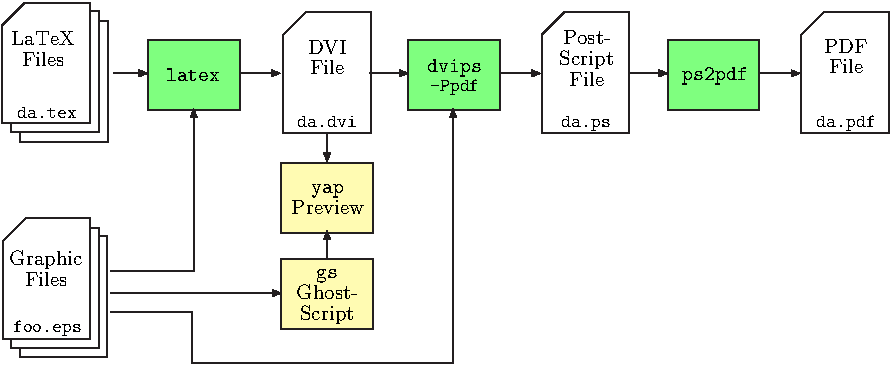
\includegraphics[width=1.0\textwidth]{workflow-cm}
\caption{Erzeugung von
PDF-Doku\-men\-ten im DVI-PS-Workflow. EPS-Grafiken werden erst bei der
Erzeugung der PS-Datei eingebunden. 
Anmerkung: Die abgebildete Vektorgrafik wurde mit \emph{Freehand} unter
Verwendung der \emph{BaKoMa} TrueType-Schriften erstellt %
(s.\ Abschn.\ \ref{sec:tex-schriften-in-grafiken}).}
\label{fig:latex-pdf-workflow}
\end{figure}

\end{comment}


\section{Drucken}

Vor dem Drucken der Arbeit empfiehlt es sich, einige Dinge zu beachten, um unnötigen Aufwand (und auch Kosten) zu vermeiden.

\subsection{Drucker und Papier}

Die Abschlussarbeit sollte in der Endfassung unbedingt auf einem
qualitativ hochwertigen Laserdrucker ausgedruckt werden, Ausdrucke
mit Tintenstrahldruckern sind \emph{nicht} ausreichend. Auch das
verwendete Papier sollte von guter Qualität (holzfrei) und
üblicher Stärke (mind.\ $80\; {\mathrm g} / {\mathrm m}^2$) sein.
Falls \emph{farbige} Seiten notwendig sind, sollte man diese einzeln%
\footnote{Tip: Mit \emph{Adobe Acrobat} lassen sich sehr einfach einzelne Seiten
des Dokuments für den Farbdruck auswählen und zusammenstellen.}
auf einem Farb-Laserdrucker ausdrucken und dem Dokument beifügen.

Übrigens sollten \emph{alle} abzugebenden Exemplare \textbf{gedruckt} (und nicht kopiert) werden! Die Kosten für den Druck
sind heute nicht höher als die für Kopien, der
Qualitätsunterschied ist jedoch -- \va\ bei Bildern und Grafiken
-- meist deutlich.


\subsection{Druckgröße}

Zunächst sollte sichergestellt werden, dass die in der fertigen PDF-Datei eingestellte
Papiergröße tatsächlich \textbf{A4} ist! Das geht \zB\ mit \emph{Adobe Acrobat}
oder \emph{SumatraPDF}
über \texttt{File} $\rightarrow$ \texttt{Properties},
wo die Papiergröße des Dokuments angezeigt wird:
\begin{center}
\textbf{Richtig:} A4 = $8{,}27 \times 11{,}69$ in \bzw\ $21{,}0 \times 29{,}7$ cm.
\end{center}
Falls das nicht stimmt, ist vermutlich irgendwo im Workflow versehentlich \textbf{Letter} 
als Papierformat eingestellt, %, häufig ist \emph{Adobe Distiller} "schuld".


Ein häufiger und leicht zu übersehender Fehler beim Ausdrucken von
PDF-Doku\-menten wird durch die versehentliche Einstellung der
Option "Fit to page" im Druckmenü verursacht, wobei die Seiten
meist zu klein ausgedruckt werden. Überprüfen Sie daher die Größe
des Ausdrucks anhand der eingestellten Zeilenlänge oder mithilfe
einer Messgrafik, wie am Ende dieses Dokuments gezeigt.
Sicherheitshalber sollte diese Messgrafik bis zur
Fertigstellung der Arbeit beibehalten und die entsprechende
Seite erst ganz am Schluss zu entfernt werden.
Wenn, wie häufig der Fall, einzelne Seiten getrennt in Farbe gedruckt 
werden, so sollten natürlich auch diese genau auf die Einhaltung der Druckgröße 
kontrolliert werden!




\section{Binden}

Die Endfassung der Abschlussarbeit%
\footnote{Für \textbf{Bachelorarbeiten} genügt, je nach Vorgaben des Studiengangs, meist eine einfache Bindung (Copyshop oder Bibliothek).}
ist in fest gebundener Form
einzureichen.%
\footnote{An der Fakultät Hagenberg ist bei Masterarbeiten zumindest eines der
Exemplare \emph{ungebunden} abzugeben -- dieses wird später von einem
Buchbinder in einheitlicher Form gebunden und verbleibt
danach in der Bibliothek. Datenträger sind bei diesem Exemplar lose 
und \emph{ohne} Aufkleber (jedoch beschriftet) beizulegen.}
Dabei ist eine Bindung zu
verwenden, die das Ausfallen von einzelnen Seiten nachhaltig
verhindert, \zB durch eine traditionelle Rückenbindung
(Buchbinder) oder durch handelsübliche Klammerungen aus Kunststoff
oder Metall. Eine einfache Leimbindung ohne Verstärkung ist
jedenfalls \emph{nicht} ausreichend.


Falls man -- was sehr zu empfehlen ist -- die Arbeit bei einem
professionellen Buchbinder durchführen lässt, sollte man auch auf
die Prägung am Buchrücken achten, die kaum zusätzliche Kosten
verursacht. Üblich ist dabei die Angabe des Familiennamens des
Autors und des Titels der Arbeit. Ist der Titel der Arbeit zu
lang, muss man notfalls eine gekürzte  Version angeben, wie \zB:
%
\begin{center}
\setlength{\fboxsep}{3mm}
\fbox{
\textsc{Schlaumeier}
\textperiodcentered\ \textsc{Part.\ Lösungen zur allg.\ Problematik}}
\end{center}
%



\section{Elektronische Datenträger (CD-R, DVD, USB-Stick)}
Speziell bei Arbeiten im Bereich der Informationstechnik (aber
nicht nur dort) fallen fast immer Informationen an, wie Programme,
Daten, Grafiken, Kopien von Internetseiten \usw, die für eine
spätere Verwendung elektronisch verfügbar sein sollten.
Vernünftigerweise wird man diese Daten während der Arbeit bereits
gezielt sammeln und der fertigen Arbeit auf einer CD-ROM, DVD oder
einem USB-Stick beilegen. Es ist außerdem sinnvoll -- schon allein
aus Gründen der elektronischen Archivierbarkeit -- die eigene Arbeit
selbst als PDF-Datei beizulegen.%
\footnote{Auch Bilder und Grafiken könnten in elektronischer Form nützlich
sein, die \latex- oder Word-Dateien sind hingegen überflüssig.}


Falls ein elektronischer Datenträger (CD-ROM, DVD, USB-Stick) beigelegt
wird, sollte auf folgende Dinge geachtet werden:
%
\begin{enumerate}
\item Jedem abzugebenden Exemplar muss eine identische Kopie des
Datenträgers beiliegen. %
\item Verwenden Sie qualitativ hochwertige Rohlinge und überprüfen
Sie nach der Fertigstellung die tatsächlich gespeicherten Inhalte
des Datenträgers! %
\item Der Datenträger sollte in eine im hinteren Umschlag
eingeklebte Hülle eingefügt sein und sollte so zu entnehmen sein,
dass die Hülle dabei \emph{nicht} zerstört wird (die
meisten Buchbinder haben geeignete Hüllen parat). %
\item Der Datenträger muss so beschriftet sein, dass er der
Abschlussarbeit eindeutig zuzuordnen ist, am Besten durch ein
gedrucktes Label%
\footnote{Nicht beim lose abgegebenen Bibliotheksexemplar --
dieses erhält ein standardisiertes Label durch die Bibliothek.} %
oder sonst durch \emph{saubere}
Beschriftung mit
der Hand und einem feinen, wasserfesten Stift. %
\item Nützlich ist auch ein (grobes) Verzeichnis der Inhalte des
Datenträgers (wie exemplarisch in Anhang \ref{app:cdrom}).
\end{enumerate}

\chapter{Schlussbemerkungen}
\label{cha:Schluss}



%%%----------------------------------------------------------
\appendix                                            % Anhang 
%%%----------------------------------------------------------

\chapter{Technische Informationen}
\label{app:TechnischeInfos}

	% Technische Ergänzungen
\chapter{Inhalt der CD-ROM/DVD}
\label{app:cdrom}

	% Inhalt der CD-ROM/DVD
\chapter{Fragebogen}
\label{app:Fragebogen}

	% Chronologische Liste der Änderungen
\chapter{\latex-Quellkode}
\label{app:Quellcode}

	% Quelltext dieses Dokuments

%%%----------------------------------------------------------
\MakeBibliography                        % Quellenverzeichnis
%%%----------------------------------------------------------

%%% Messbox zur Druckkontrolle ------------------------------
\chapter*{Messbox zur Druckkontrolle}



\begin{center}
{\Large --- Druckgröße kontrollieren! ---}

\bigskip

\calibrationbox{100}{50} % Angabe der Breite/Hoehe in mm

\bigskip

{\Large --- Diese Seite nach dem Druck entfernen! ---}

\end{center}



%%%----------------------------------------------------------
\end{document}
%%%----------------------------------------------------------